%角动量加法

\pentry{轨道角动量, 张量积空间\upref{DirPro}}

考虑两个系统的角动量空间, 基底分别为 $\ket{l_1, m_1}$ 和 $\ket{l_2, m_2}$, 其中 $l_1, l_2$ 固定空间的维度分别为 $2l_1+1$ 和 $2l_2+1$. 两空间的角动量算符分别为
\begin{equation}
L_1^2 \qquad L_{1x} \qquad L_{1y} \qquad L_{1z}
\end{equation}
\begin{equation}
L_2^2 \qquad L_{2x} \qquad L_{2y} \qquad L_{2z}
\end{equation}

我们用这两个空间生成 $(2l_1+1)(2l_2+1)$ 维的张量积空间, 基底为 $\ket{l_1, m_1} \ket{l_2, m_2}$ (或记为 $\ket{l_1, m_1, l_2, m2}$). 张量积空间中一组显然的 Complete Set of Commutable Operators (CSCO)为
\begin{equation}
\{L_{1z}, L_{2z}\}
\end{equation}

在张量积空间上定义两个系统总角动量算符为
\begin{equation}
L_x = L_{1x} \oplus L_{2x}
\qquad
L_y = L_{1y} \oplus L_{2y}
\qquad
L_z = L_{1z} \oplus L_{2z}
\end{equation}
\begin{equation}
J^2 = L_x^2 + L_y^2 + L_z^2
\end{equation}
可以证明新增的对易关系为
\begin{equation}
\comm*{J^2}{J_z} = \comm*{J^2}{L_1^2} = \comm*{J^2}{L_2^2} = 
\comm*{J_z}{L_{1z}} = \comm*{J_z}{L_{2z}} = 0
\end{equation}
由此可以得到另一组 CSCO 为 %未完成:如何得到?
\begin{equation}
\{J^2, J_z\}
\end{equation}
即我们可以想得到张量积空间的另一组基底. 令两个算符的本征值(量子数)分别为 $J$  和 $M$, 这组基底可记为 $\ket{J, M}$.  首先由对易关系, $\ket{l_1, m_1, l_2, m_2}$ 已经是 $J_z$ 的本征矢,每个本征值 $M$ 对应一个子空间(因为有简并). 子空间的维数 $N_M$ 是 $m_1 + m_2 = M$ 的不同组合数(\autoref{AMAdd_fig1} 左). 例如图中当 $M = l_1 + l_2 = 7/2$ 时 $N_M = 1$ (唯一的非简并情况), $M = -1/2$ 时 $N_M = 4$.
\begin{figure}[ht]
\centering
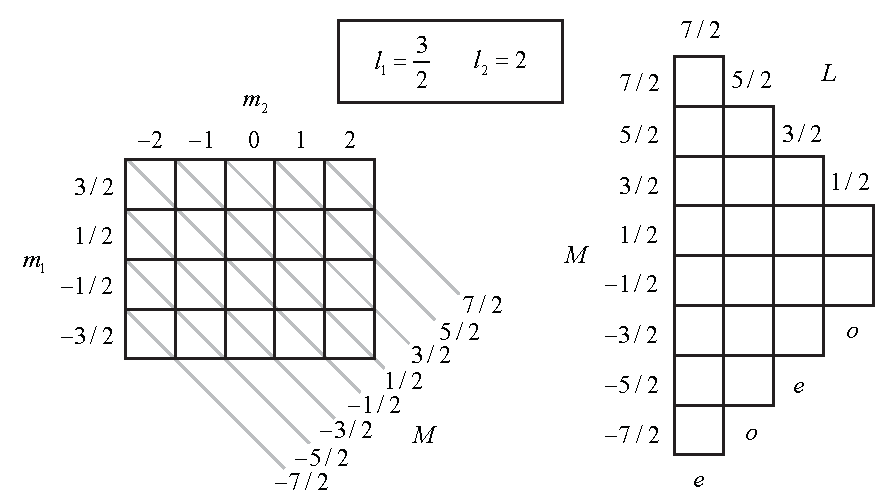
\includegraphics[width=14cm]{./figures/AMAdd1.pdf}
\caption{图中每个方格代表一个基底. 这个空间也可以使用 $\ket{L, M}$ 作为基底, 且基底变换在每个 $M$ 子空间中独立进行} \label{AMAdd_fig1}
\end{figure}

\begin{equation}
N_M = \leftgroup{
&l_1 + l_2 - \abs{M} + 1 \quad& &(\abs{M} > \abs{l_1 - l_2}) \\
&\min\{l_1, l_2\} \quad & &(\abs{M} \les \abs{l_1 - l_2})
}\end{equation}
我们只需要在每个 $M$ 子空间中把 $J^2$ 算符对角化即可.
\begin{equation}
J^2 = L_1^2 + L_2^2 + 2(L_{1x} L_{2x} + L_{1y} L_{2y} + L_{1z} L_{2z})
\end{equation}
其中只有 $L_{1x} L_{2x} + L_{1y} L_{2y}$  不是对角矩阵.利用升降算符表示
\begin{equation}
2 (L_{1x} L_{2x} + L_{1y} L_{2y} ) = L_{1+} L_{2-} + L_{1-} L_{2+}
\end{equation} 
\begin{equation}\ali{
&\quad \bra{l_1, m'_1, l_2, m'_2} J^2 \ket{l_1, m_1, l_2, m_2}\\
&= \hbar ^2 \qty[ \ali{
&\delta_{m'_1, m_1} \delta_{m'_2, m_2} [l_1(l_1 + 1) + l_2(l_2 + 1) + 2 m_1 m_2]  \\
+ &\delta_{m'_1, m_1 + 1} \delta_{m'_2, m_2 - 1} \sqrt{l_1 (l_1 + 1) - m_1(m_1 + 1)} \sqrt{l_2 (l_2 + 1) - m_2(m_2 - 1)}\\
+ &\delta_{m'_1, m_1 - 1} \delta_{m'_2, m_2 + 1} \sqrt{l_1 (l_1 + 1) - m_1(m_1 - 1)} \sqrt{l_2 (l_2 + 1) - m_2(m_2 + 1)} }]
}\end{equation}
 
矩阵的具体形式取决于基底的排列顺序. 把$\ket{J,M}$ 以 $J$ 从大到小的顺序排列, 基底 $\ket{l_1, m_1, l_2, m_2}$ ($m_2 = M - m_1$)以 $m_1$ 从大到小的顺序排列. 每组基底中 $m_1$ 的最大值为
\begin{equation}
\max \qty{m_1} = \leftgroup{
&l_1 \quad& &(M \ges l_1 - l_2)  \\
&l_2 + M & &(M < l_1 - l_2)
}\end{equation}
这样, $J^2$ 的矩阵就是一个三对角矩阵,其本征矢矩阵就是从 $\ket{J, M}$ 表象到 $\ket{l_1, m_1, l_2, m_2}$ 表象的幺正变换矩阵 $\mat U_M$.

查 CG 表时, CG 系数通常以 $\mat U_M$ 矩阵的形式给出(如 Griffiths).可以证明, $\mat U_M$ 的 $N_M$ 个本征值为 $J(J + 1) \hbar ^2$,  其中 $J = l_1 + l_2, l_1 + l_2 - 1,\dots$ (共 $N$ 项%未完成,不会证明
)(注意最小值大于但不一定等于 $\abs{M}$ ). $J$ 在所有子空间的最小值是 $\abs{l_1 - l_2}$ (当 $\abs{M} = \abs{l_1 - l_2}$ 时取得),所以 $J$ 在所有子空间的范围是
\begin{equation}
J = \abs{l_1 - l_2}, \dots, l_1 + l_2
\end{equation}
现在我们已经知道了每个子空间 $M$ 的变换,那么如何求总变换呢?先把总矩阵列表,行标题是所有的 $\ket{l_1, m_1} \ket{l_2, m_2}$, 列标题是所有的 $\ket{J, M}$, 对每个空间,找到对应的 $N$ 行和 $N$ 列,把 $N \times N$  的 $\mat U_M$ 矩阵照抄上去即可.

%未完成: 图中的 e 和 o 代表粒子交换的对称性, 推导一下为什么会是交替出现.
